\documentclass[tikz,border=2pt]{standalone}

\usepackage[T1]{fontenc}
\usepackage{newtxtext,newtxmath}
% newtxmath defines \Bbbk before amssymb on this TeX Live build.
\let\Bbbk\relax
\usepackage{amsmath,amssymb,bm}
\usepackage{tikz}
\usepackage{pgfplots}

\usetikzlibrary{
  arrows.meta,
  positioning,
  fit,
  calc,
  backgrounds,
  shapes.geometric,
  shapes.multipart,
  matrix
}

\pgfplotsset{compat=1.18}

\definecolor{FigTeal}{HTML}{539F97}
\definecolor{FigBlue}{HTML}{6C7AAD}
\definecolor{FigRose}{HTML}{BE7A7A}
\definecolor{FigDark}{HTML}{252525}
\definecolor{FigGrid}{HTML}{E7EBEF}
\definecolor{FigNeutral}{HTML}{F5F4F0}
\definecolor{FigLightTeal}{HTML}{DDECEA}
\definecolor{FigLightBlue}{HTML}{E3E6F0}
\definecolor{FigLightRose}{HTML}{F0DFDF}

\newcommand{\grouptitlefont}{\fontsize{8.4}{9.6}\selectfont\bfseries}
\newcommand{\boxtitlefont}{\fontsize{8.0}{9.0}\selectfont\bfseries}
\newcommand{\normalfontsmall}{\fontsize{7.2}{8.1}\selectfont}
\newcommand{\eqfont}{\fontsize{7.2}{8.1}\selectfont}
\newcommand{\legendfont}{\fontsize{6.9}{7.7}\selectfont}
\newcommand{\labelfontsmall}{\fontsize{6.9}{7.7}\selectfont}

\tikzset{
  basebox/.style={
    rounded corners=2pt,
    draw=FigDark,
    line width=0.75pt,
    align=center,
    inner sep=4pt
  },
  actorbox/.style={
    basebox,
    draw=FigBlue,
    fill=FigLightBlue
  },
  criticbox/.style={
    basebox,
    draw=FigTeal,
    fill=FigLightTeal
  },
  targetactor/.style={
    actorbox,
    dashed
  },
  targetcritic/.style={
    criticbox,
    dashed
  },
  replaybox/.style={
    basebox,
    draw=FigDark,
    fill=FigNeutral
  },
  updatebox/.style={
    basebox,
    draw=FigRose,
    fill=FigLightRose
  },
  legendbox/.style={
    basebox,
    draw=FigDark,
    fill=FigNeutral
  },
  groupbox/.style={
    rounded corners=2pt,
    draw=FigGrid,
    line width=0.65pt,
    fill=white
  },
  dataflow/.style={
    -{Latex[length=2.0mm,width=1.2mm]},
    draw=FigDark,
    line width=0.9pt
  },
  gradflow/.style={
    -{Latex[length=2.0mm,width=1.2mm]},
    draw=FigRose,
    dashed,
    line width=0.85pt
  },
  softflow/.style={
    -{Latex[length=2.0mm,width=1.2mm]},
    draw=gray!75!black,
    dash dot,
    line width=0.8pt
  },
  arrowlabel/.style={
    fill=white,
    inner sep=1.2pt,
    font=\labelfontsmall,
    text=FigDark
  },
  legendtext/.style={
    font=\legendfont,
    text=FigDark
  },
  grouptitle/.style={
    font=\grouptitlefont,
    text=FigDark
  }
}

\begin{document}
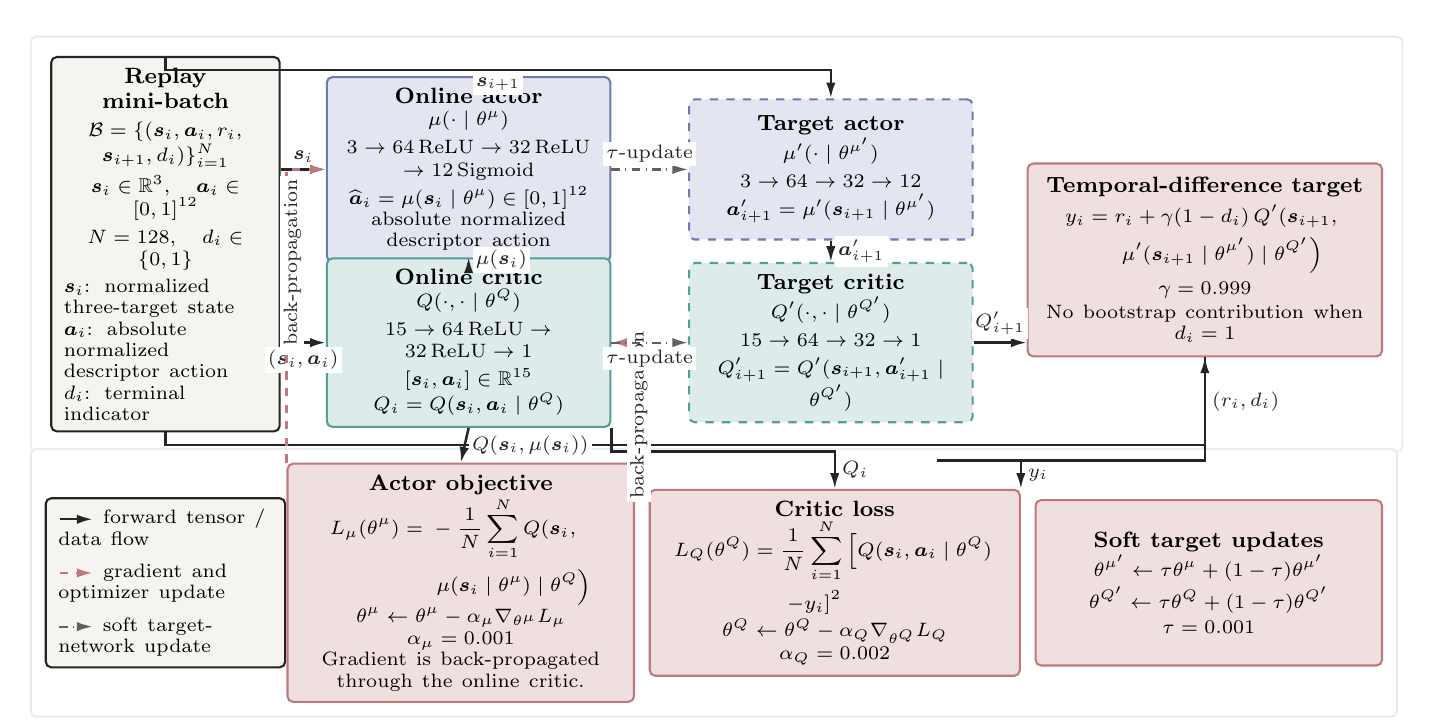
\begin{tikzpicture}[x=1cm,y=1cm]
\path[use as bounding box] (0,0) rectangle (17.5,8.5);

\node[replaybox, minimum width=2.9cm, minimum height=3.9cm, text width=2.62cm] (replay) at (1.75,5.75) {%
  \begin{minipage}{2.58cm}\centering
  {\boxtitlefont Replay mini-batch\par}
  \vspace{2pt}
  {\eqfont
  $\mathcal B=\{(\bm s_i,\bm a_i,r_i,$\par
  $\bm s_{i+1},d_i)\}_{i=1}^{N}$\par
  \vspace{2pt}
  $\bm s_i\in\mathbb R^3,\quad \bm a_i\in[0,1]^{12}$\par
  \vspace{2pt}
  $N=128,\quad d_i\in\{0,1\}$\par}
  \vspace{2pt}
  {\legendfont\raggedright
  $\bm s_i$: normalized three-target state\par
  $\bm a_i$: absolute normalized descriptor action\par
  $d_i$: terminal indicator\par}
  \end{minipage}
};

\node[actorbox, minimum width=3.6cm, minimum height=1.78cm, text width=3.32cm] (onlineactor) at (5.6,6.70) {%
  \begin{minipage}{3.28cm}\centering
  {\boxtitlefont Online actor\par}
  {\eqfont $\mu(\cdot\mid\theta^\mu)$\par}
  \vspace{2pt}
  {\eqfont $3\to64\,\mathrm{ReLU}\to32\,\mathrm{ReLU}$\par
  $\to12\,\mathrm{Sigmoid}$\par}
  \vspace{2pt}
  {\eqfont $\widehat{\bm a}_i=\mu(\bm s_i\mid\theta^\mu)\in[0,1]^{12}$\par}
  {\legendfont absolute normalized descriptor action\par}
  \end{minipage}
};

\node[criticbox, minimum width=3.6cm, minimum height=1.78cm, text width=3.32cm] (onlinecritic) at (5.6,4.50) {%
  \begin{minipage}{3.28cm}\centering
  {\boxtitlefont Online critic\par}
  {\eqfont $Q(\cdot,\cdot\mid\theta^Q)$\par}
  \vspace{2pt}
  {\eqfont $15\to64\,\mathrm{ReLU}\to32\,\mathrm{ReLU}\to1$\par}
  \vspace{2pt}
  {\eqfont $[\bm s_i,\bm a_i]\in\mathbb R^{15}$\par
  $Q_i=Q(\bm s_i,\bm a_i\mid\theta^Q)$\par}
  \end{minipage}
};

\node[targetactor, minimum width=3.6cm, minimum height=1.78cm, text width=3.32cm] (targetactor) at (10.20,6.70) {%
  \begin{minipage}{3.28cm}\centering
  {\boxtitlefont Target actor\par}
  {\eqfont $\mu'(\cdot\mid\theta^{\mu'})$\par}
  \vspace{2pt}
  {\eqfont $3\to64\to32\to12$\par}
  \vspace{2pt}
  {\eqfont $\bm a^{\prime}_{i+1}=\mu'(\bm s_{i+1}\mid\theta^{\mu'})$\par}
  \end{minipage}
};

\node[targetcritic, minimum width=3.6cm, minimum height=1.78cm, text width=3.32cm] (targetcritic) at (10.20,4.50) {%
  \begin{minipage}{3.28cm}\centering
  {\boxtitlefont Target critic\par}
  {\eqfont $Q'(\cdot,\cdot\mid\theta^{Q'})$\par}
  \vspace{2pt}
  {\eqfont $15\to64\to32\to1$\par}
  \vspace{2pt}
  {\eqfont
  $Q'_{i+1}=Q'(\bm s_{i+1},\bm a^{\prime}_{i+1}\mid\theta^{Q'})$\par}
  \end{minipage}
};

\node[updatebox, minimum width=4.5cm, minimum height=2.45cm, text width=4.16cm] (tdtarget) at (14.95,5.55) {%
  \begin{minipage}{4.12cm}\centering
  {\boxtitlefont Temporal-difference target\par}
  \vspace{2pt}
  {\eqfont
  $\begin{aligned}
  y_i={}&r_i+\gamma(1-d_i)\,
  Q'\!\left(\bm s_{i+1},\right.\\[-1pt]
  &\left.\mu'(\bm s_{i+1}\mid\theta^{\mu'})
  \mid\theta^{Q'}\right)
  \end{aligned}$\par
  \vspace{2pt}
  $\gamma=0.999$\par}
  \vspace{1pt}
  {\legendfont No bootstrap contribution when $d_i=1$\par}
  \end{minipage}
};

\node[legendbox, minimum width=3.0cm, minimum height=1.55cm, text width=2.76cm] (legend) at (1.75,1.45) {%
  \begin{minipage}{2.72cm}
  {\legendfont
  \tikz[baseline=-0.55ex]{\draw[dataflow] (0,0)--(0.42,0);} forward tensor / data flow\par
  \vspace{4pt}
  \tikz[baseline=-0.55ex]{\draw[gradflow] (0,0)--(0.42,0);} gradient and optimizer update\par
  \vspace{4pt}
  \tikz[baseline=-0.55ex]{\draw[softflow] (0,0)--(0.42,0);} soft target-network update\par}
  \end{minipage}
};

\node[updatebox, minimum width=4.4cm, minimum height=2.1cm, text width=4.05cm] (actorobj) at (5.50,1.45) {%
  \begin{minipage}{4.00cm}\centering
  {\boxtitlefont Actor objective\par}
  {\eqfont
  $\begin{aligned}
  L_\mu(\theta^\mu)={}&-\frac{1}{N}\sum_{i=1}^{N}
  Q\!\left(\bm s_i,\right.\\[-1pt]
  &\left.\mu(\bm s_i\mid\theta^\mu)\mid\theta^Q\right)
  \end{aligned}$\par
  $\theta^\mu\leftarrow\theta^\mu-\alpha_\mu\nabla_{\theta^\mu}L_\mu$\par
  $\alpha_\mu=0.001$\par}
  {\legendfont Gradient is back-propagated through the online critic.\par}
  \end{minipage}
};

\node[updatebox, minimum width=4.7cm, minimum height=2.1cm, text width=4.34cm] (criticloss) at (10.25,1.45) {%
  \begin{minipage}{4.30cm}\centering
  {\boxtitlefont Critic loss\par}
  {\eqfont
  $\begin{aligned}
  L_Q(\theta^Q)={}&\frac{1}{N}\sum_{i=1}^{N}
  \left[Q(\bm s_i,\bm a_i\mid\theta^Q)\right.\\[-1pt]
  &\left.-y_i\right]^2
  \end{aligned}$\par
  $\theta^Q\leftarrow\theta^Q-\alpha_Q\nabla_{\theta^Q}L_Q$\par
  $\alpha_Q=0.002$\par}
  \end{minipage}
};

\node[updatebox, minimum width=4.4cm, minimum height=2.1cm, text width=4.05cm] (softupdate) at (15.00,1.45) {%
  \begin{minipage}{4.00cm}\centering
  {\boxtitlefont Soft target updates\par}
  {\eqfont
  $\theta^{\mu'}\leftarrow\tau\theta^\mu+(1-\tau)\theta^{\mu'}$\par
  \vspace{1pt}
  $\theta^{Q'}\leftarrow\tau\theta^Q+(1-\tau)\theta^{Q'}$\par
  \vspace{1pt}
  $\tau=0.001$\par}
  \end{minipage}
};

\begin{scope}[on background layer]
  \node[groupbox, fit=(replay)(onlineactor)(onlinecritic)(targetactor)(targetcritic)(tdtarget), inner sep=7pt] {};
  \node[groupbox, fit=(legend)(actorobj)(criticloss)(softupdate), inner sep=5pt] {};
\end{scope}

\draw[dataflow] (replay.east |- onlineactor.west) -- node[arrowlabel, above=1pt] {$\bm s_i$} (onlineactor.west);
\draw[dataflow] (replay.east |- onlinecritic.west) -- node[arrowlabel, below=1pt] {$(\bm s_i,\bm a_i)$} (onlinecritic.west);
\draw[dataflow] (onlineactor.south) -- node[arrowlabel, right=1pt] {$\mu(\bm s_i)$} (onlinecritic.north);

\draw[dataflow] (replay.north) -- (1.75,7.96) -- node[arrowlabel, below=1pt] {$\bm s_{i+1}$} (10.20,7.96) -- (targetactor.north);
\draw[dataflow] (targetactor.south) -- node[arrowlabel, right=1pt] {$\bm a^{\prime}_{i+1}$} (targetcritic.north);
\draw[dataflow] (replay.south) |- (13.05,3.20) -| node[arrowlabel, near end, right=1pt] {$(r_i,d_i)$} (tdtarget.south);
\draw[dataflow] (targetcritic.east) -- node[arrowlabel, above=1pt] {$Q'_{i+1}$} (tdtarget.west |- targetcritic.east);

\draw[dataflow] (onlinecritic.south) -- node[arrowlabel, right=1pt] {$Q(\bm s_i,\mu(\bm s_i))$} (actorobj.north);
\draw[dataflow] (onlinecritic.south east) |- (8.15,3.12) -| node[arrowlabel, near end, right=1pt] {$Q_i$} (criticloss.north);
\draw[dataflow] (tdtarget.south) |- (11.55,3.00) -| node[arrowlabel, near end, right=1pt] {$y_i$} (criticloss.north east);

\draw[gradflow] (actorobj.north west) |- (3.45,6.70) -- (onlineactor.west);
\node[arrowlabel, rotate=90] at (3.36,5.52) {back-propagation};
\draw[gradflow] (criticloss.north west) |- (7.65,4.50) -- (onlinecritic.east);
\node[arrowlabel, rotate=90] at (7.76,3.58) {back-propagation};

\draw[softflow] (onlineactor.east) -- node[arrowlabel, above=1pt] {$\tau$-update} (targetactor.west);
\draw[softflow] (onlinecritic.east) -- node[arrowlabel, below=1pt] {$\tau$-update} (targetcritic.west);

\end{tikzpicture}
\end{document}
